\documentclass[phd,tocprelim]{cornell}
\let\ifpdf\relax
%
% tocprelim option must be included to put the roman numeral pages in the
% table of contents
%
% The cornellheadings option will make headings completely consistent with
% guidelines.
%
% This sample document was originally provided by Blake Jacquot, and
% fixed up by Andrew Myers.
%
% ************* TODO (Brandon Barker) ***********************************

%General
% Figure out the best way to modularize chapters/sections in different files.
%
% Verify bibliography working; check eMoMA script and add to Makefile?
%
% Appendix can work as a place for supplementary notes and figures?
%
% Semi-automate Mendeley->.bib citation process
% TODO (Brandon Barker)
% Read Formatting Rules on Grad School site.
%  - referencing figures/capitalization: Fig or fig or figure ...
%
% Spellcheck
%
% Permissions: Once title of thesis is known, write permission letter to use publications
% http://www.proquest.com/assets/downloads/products/UMI_CopyrightGuide.pdf
%
% Word histogram to check for words used too often.
%

% Chapter 1: Introduction:
% Add other (Jason-deleted) sections/words
% Refs/Figs
% Epistasis

% Chapter 3: 
%
% Consider adding the Motif/model work somehow


%Chapter 4:
%
% Tie in motivating rules example with previous section
% showing the merits of CNF
%
% Add another illustrative figure.
%
% Add a table/figure comparing estimated EC abundance using
% e.g. original method vs our method, also for fluxes.
% - Benchmark these against cancer data in Chapter 5
%
% Figure out how copyright registration is handled; apparently it is necesasry.
% I assume it is handled by Cornell.
%

% ************* End of TODO ***********************************************
%Added by Brandon:
\usepackage{soul} %For highlights
\usepackage{amsmath}
\usepackage{hyperref}
\usepackage{float}
\usepackage{tikz}
\usepackage{algorithmic}
\usepackage[amsmath,amsthm,thmmarks]{ntheorem}

%Some possible packages to include
\usepackage{graphicx,pstricks}
\usepackage{graphics}
\usepackage{moreverb}
\usepackage{subfigure}
\usepackage{epsfig}
\usepackage{subfigure}
\usepackage{hangcaption}
\usepackage{txfonts}
\usepackage{palatino}

\graphicspath{{./figures/}}
\usetikzlibrary{shapes,arrows}

%if you're having problems with overfull boxes, you may need to increase
%the tolerance to 9999
\tolerance=9999

\bibliographystyle{plain}
%\bibliographystyle{IEEEbib}

\renewcommand{\caption}[1]{\singlespacing\hangcaption{#1}\normalspacing}
\renewcommand{\topfraction}{0.85}
\renewcommand{\textfraction}{0.1}
\renewcommand{\floatpagefraction}{0.75}

\title {Advances in Genome-Scale Metabolic Models Applied to Adaptive and Environmental Epistatic Landscapes and Cancer Physiology}
\author {Brandon Barker}
\conferraldate {August}{2013}
\degreefield {Ph.D.}
\copyrightholder{Brandon Elam Barker}
\copyrightyear{2013}

\renewcommand{\algorithmicrequire}{\textbf{Input:}}
\renewcommand{\algorithmicensure}{\textbf{Output:}}

\newtheorem{Theorem}{Theorem}
\theoremstyle{break}
\newtheorem{Algorithm}{Algorithm}
\theoremstyle{empty}
\newtheorem{assume}{}

\begin{document}
% Define block styles
\tikzstyle{decision} = [diamond, draw, fill=blue!20,
    text width=4.5em, text badly centered, node distance=3cm, inner sep=0pt]
\tikzstyle{block} = [rectangle, draw, fill=blue!20,
    text width=5em, text centered, node distance=3cm, minimum height=4em]
\tikzstyle{line} = [draw, very thick, color=black!50, -latex']
\tikzstyle{cloud} = [draw, ellipse,fill=red!20, node distance=3cm,
    minimum height=2em]
\tikzstyle{iogram} = [trapezium, draw, fill=pink!20,
    trapezium left angle=70,trapezium right angle=-70, inner xsep=0pt,
    text width=5em, text centered, node distance=3cm, minimum height=4em]


\maketitle
\makecopyright

\begin{abstract}

There has been a surge of interest in understanding the regulation 
of metabolic networks involved in disease in recent years.  Quantitative 
models are increasingly being used to interrogate the metabolic pathways 
that are contained within this complex disease biology.  At the core of 
this effort is the mathematical modeling of central carbon metabolism involving 
glycolysis and the citric acid cycle (referred to as energy metabolism).  
Here we discuss several approaches used to quantitatively model metabolic 
pathways relating to energy metabolism and discuss their formalisms, successes, and limitations.
Your abstract goes here. Make sure it sits inside the brackets. If not,
your biosketch page may not be roman numeral iii, as required by the
graduate school.
\end{abstract}

\begin{biosketch}
Your biosketch goes here. Make sure it sits inside
the brackets.
\end{biosketch}

\begin{dedication}
\begin{center}
\textit{To my parents---James and Carol Barker, \\
For their love, time, and beneficence, \\
Without which this work would not have been possible. \\
\vspace{10 mm} 
To my wife, Lin Xue, \\
For giving me the mommentum to pursue graduate school, \\
For her patience while I studied, \\
For her continuing love and , \\
And most importantly, for being an amazing mother.\\
\vspace{10 mm} 
To my son, Lindon Barker, \\
For your extra motivation towards finishing in a timely manner, \\
And for your terrific smiles, grins, and laughs during this last year.}
\end{center}
\end{dedication}

\begin{acknowledgements}
Firstly I would like to thank my advisor, Dr. Zhenglong Gu, under
whose supervision this work has unfolded, and who has provided me with
substantial support, encouragement, and irreplacable mentoring. I owe
much to my colleague and friend, Dr. Lin Xu, for not only showing me
the ropes and giving me hope, but also getting me interested in so
many topics in evolution; much of the present work, particularly that
involving epistasis, would not have happened without him. Without
Dr. Jason Locasale's intellectual incitation and advise, I never would
have wandered down the path to what has, to me, become the most
interesting part of this work, nor the path to the Big Red Barn quite
so much as I did. My thesis committee members---Dr. David Christini,
Dr. Chris Myers, and Dr. Michael Stillman---have provided much advice
over the years, scientific and otherwise.

My other collaborators in the present work include Dr. Tim Connallon,
whose knowledge on epistasis surpasses anyone I know, and similarly
for Dr. Alex Shestov with regard to metabolic flux analysis;
Dr. Kieran Smallbone, who has given helpful advice over the years 
regarding constraint-based models, as well as having helped develop several  
algorithms and models that I have employed in this work, including one in 
particular that served as the impetus for some of the research in the latter 
chapters; Mr. Yiping Wang, a phenomenal young researcher who helped
with some analysis in the last chapter during his first month on
campus, and Dr. Hongwei Xi, for providing substantial support for his
programming language ATS, which was employed in the latter chapters.

In the lab, Dr. Xiaoxian Guo, Dr. Huifeng Jiang, and Dr. Zhe Wang
provided much experimental advice, training, and data.

I would also like to thank many other colleagues for their help,
friendship, scientific discussion, or some combination of
the three. These include Ms. Diana Chang, Mr. Elijah Bogart, 
Dr. Hong Chian, Dr. Martha Field, Mr. Lei Huang,
Ms. Haley Hunter-Zinck, Dr. Ben Heavner, Dr. Xiaojing Liu, Ms. Anuttama Mohan,
Mr. Lonnie Princehouse, Mr. Narayanan Sadagopan, and Mr. Kaixiong Ye.

Without the stimulus, confidence, and aid from my early mentors at the
University of Kentucky, this document would not exist; in particular,
I thank Dr. Ruriko Yoshida, for renewing my passion in science,
Dr. Jim Lund, for being my first biology mentor (and providing the
opportunity to become acquainted with my wife), Dr. Jerzy Jaromczyk
for his friendly help and advice throughout and beyond my
undergraduate education, and to Dr. Henry Dietz, for being a great
educator and advising my senior design project.  My passionate and
reassuring high school biology teacher, Mr. David Christiansen,
warrants special thanks for being continually amazed at the wonders
biology has to offer. Lastly, I thank my friend Mr. Benjamin Runyon,
for always lending an ear.
\end{acknowledgements}

\contentspage
\tablelistpage
\figurelistpage

\normalspacing \setcounter{page}{1} \pagenumbering{arabic}
\pagestyle{cornell} \addtolength{\parskip}{0.5\baselineskip}

\chapter{Introduction}

The accumulated amount of biochemical work carried out over the years
has elaborated complex metabolic systems and networks.  This
information includes the network architecture encoded in chemical
reactions that are carried out by metabolic enzymes and the kinetic
parameters that determine reaction mechanisms involved in each of
these chemical reactions.  Application of this knowledge has led to
tremendous predictive capability in characterizing metabolic
regulation in normal physiology including the growth of unicellular
organisms and the successful simulation of energy metabolism in
healthy red blood cells.  However, there are far fewer instances in
which these models have been applied to the characterization of
pathophysiology.  Applying our knowledge of metabolic regulation to
the investigation of disease states such as cancer or
neurodegeneration is currently a scientific frontier.  In this review,
we will revisit several classic techniques for the mathematical
modeling of metabolic pathways and discuss instances where their
application to biomedical science is beginning to yield fruitful
dividends.

\section{Linear Systems, Flux Balance Analysis}
Linear models are mathematical models that containt a set of algebraic
equations based on the stoichiometric relationships that define
conservation relationships within a metabolic network.  Linear models,
to our knowledge, were first applied to biochemical systems in 1961 by
Howard Shapiro1. Shapiro discussed the possibility of using
optimization in biochemical linear models in a 1969 publication2. In
1984, a model incorporating glycolysis and the TCA cycle was employed
running a variant of Dantzig’s algorithm with the assumed biological
objective of minimized free energy dissipation3,4. An enduring
research program was initiated by Bernhard Palsson half a decade
later5,6.  An early work of Palsson showed that growth maximization in
an E. coli model could correctly match 86\% of 79 gene essentialities
examined7. Subsequent modeling in S. cerevisiae was able to closely
predict growth rates and exometabolic fluxes in various media, and
nearly capture the in vivo phosphate/oxygen (P/O) ratio of 0.94 with a
simulated P/O value of 1.04, showing that models of eukaryotes were
also feasible8. If one chooses the biological objective function to
reflect the appropriate physiological demands then it is possible to
predict features of adaptation; this was shown to be the case for
growth optimization in several E. coli mutants9. By this time it had
become apparent that linear models held much promise, particularly
when coupled with optimization.


\section{Genome Scale Modeling}
Today, when we refer to linear models, we most often mean Constraint
Based Models (CBMs). We refer to a CBM as any model making use of the
stoichiometric matrix, S, as a linear matrix constraint, e.g. S * F =
0, where F is a flux vector. In fact, this is a nearly universal
constraint, as it guarantees conservation of mass during steady state
processes such as exponential growth or tissue maintenance10. Other
constraints commonly used include reversibility constraints when the
direction of a reaction is known for physiological conditions of
interest, bounds on the uptake of nutrients or efflux rates due to
regulation or physiology, or bounds on enzyme reactions when the
maximum enzyme velocity Vmax is known.

Because these constraints give rise to an underdetermined system, it
will not be possible to identify a unique solution for the flux
vector. A unique solution is often desirable as it allows
investigators to analyze a putative metabolic phenotype. Indeed, this
is one of the more convenient features of linear optimization: the
ability to get meaningful solutions without explicitly taking into
account any, or at least very few, free parameters.  Flux Balance
Analysis, or FBA, assumes a linear combination of fluxes to be
maximized or minimized (Fig 1). In microbes, perhaps the most popular
FBA objective has been growth maximization, which consists of the
biomass precursors and products formulated as a single
pseudo-reaction. Additionally, an ATP maintenance constraint should be
formulated as a sink reaction with the molar ATP required to keep one
gram of dry weight biomass living for one hour11. This empirically
determined constraint, although assumed, is less discussed, perhaps
due to its dependence on individual strains and environments.  We note
that for many expression-based methods in the CBM framework, the ATP
maintenance constraint is not required (see Table and Fig 2 for
examples). Fixed biomass objectives by themselves also have some
undesirable qualities; biomass composition likely has some measure of
variability based on genetic background and environment.  Robust FBA
attempts to address this problem by allowing some variation in the
biomass composition, as determined by variation of empirical assays of
biomass 12.  Despite these caveats, FBA has recently been found to not
only predict growth in microbes, but also has good agreement with gold
standard 13C flux assays in vivo when the growth objective is used
along with ATP synthesis maximization and minimization of absolute
fluxes13.

Minimization of absolute flux is a commonly used objective employed
alongside other objectives, forming a minimax problem (i.e. finding
the minimum absolute flux profile among all flux profiles that
maximize biomass). This approximates the biological goal of being
efficient with enzyme production costs and enzyme crowding constraints
while also guaranteeing that no thermodynamically impossible loops are
present, that is, ruling out some fluxes that might otherwise violate
Kirchoff’s loop rule14,15.  This constraint will work whenever a sink
reaction, such as growth, is being optimized.  However, maximizing an
internal flux, as in Flux Variability Analysis16, could still result
in internal cycles15. Initial thermodynamic approaches involved
nonlinear optimization17–20.  Constraints satisfying Kirchoff’s loop
rule were later developed that were faster and more generally
applicable than prior methods15,21.  Still, these involve integer
constraints that put this problem in a slower class of algorithms than
the convex minimized absolute flux problem.  When available,
thermodynamic data is valuable; it can not only be used to guarantee
there are no internal cycles, but can also aid in determining reaction
direction and potential regulatory targets15,18,22,23. Application of
this framework to concentration data allows unmeasured metabolite
concentrations to be inferred and global concentrations to be resolved
at the organelle level20. CBMs have also found use in tracing
individual atoms through pathways, which provides a more appealing
framework for performing Metabolic Flux Analysis (MFA; discussed
below) on stable isotope data due to the lack of bias compared to
typical MFA models, which are often an order of magnitude smaller than
genome-scale reconstructions24.  Recent insightful work has made it
possible to simplify the computational complexity of loopless FBA to
be nearly the same as conventional FBA, but some mathematical
difficulties must still be overcome before bounds on exchange fluxes
can be suitably incorporated for genome-scale modeling10,25.


The metabolism of different tissues within the same organism is
diverse; whereas the metabolism in liver is anabolic, neurons or red
blood cells have a much more limited catabolic regime26–28.The
creation of tissue specific models for multicellular organism has
become an important problem, and several automated algorithms taking
as inputs tissue expression data and a generic model for the organism
have been developed28–30. Coupling multiple cellular models together
will enable multi-scale modeling of tissues in multicellular models or
entire ecosystems for microbes26,31–33.

Automated generation of metabolic networks from genome sequence and
pathway databases, especially in prokaryotes, has been developed34–37.
This will offer many advantages to modelers: a starting point for
curated models (a draft reconstruction is estimated to often take
several months even in prokaryotes), a means for doing population or
ecological simulation33, and personalized genomic modeling for
patients with metabolic syndromes such as cancer where both the
patient and possibly the disease have diverse genotypes38,39.
Eukaryotic models are somewhat more difficult to generate due to the
necessity of protein localization and metabolite transporter
information34. Automatic reconstruction going beyond enzymatic gene
information, such as rFBA models, should also be possible40,41; the
automated generation of Boolean and higher-order discrete regulatory
models using time-series expression data has been explored as well,
though to date these regulatory models have not been coupled to
metabolic reconstructions42–45. These approaches and other families of
genome-scale methods are discussed in Table 1.

Several approaches have been used in applying CBMs to cancer and the
Warburg effect, the preference for glycolytic ATP production over
glucose-derived mitochondrial ATP production in cancer cells46–48. An
important study working with a simplified, small model of
central-carbon metabolism showed that, while the TCA cycle predicts
better ATP yield than glycolysis when only available glucose is
considered as a constraint, the addition of enzyme solvent-capacity
constraints creates a preference for ATP synthesis through
glycolysis48. More recently, the work of Vazquez et al. was extended
to include a genome-scale model along with enzyme solvent-capacity
constraints, which was able to show significant correlations between
fluxes and expression in the NCI-60 cell line panel, as well as
predicting an intermediate state in cancer metabolism transition
exhibiting a temporary increase in OxPhos that was supported by two
prior experimental observations47. All of these approaches correctly
predicted lactate production. Concurrent research on predicting cancer
targets by screening for simulated negative epistasis in cancer
tissue-specific models that have at least one known-drug target and no
known effect on normal tissue revealed many epistatic
interactions39. A related study confirmed one of these synthetic
lethalities between hemeoxygenase and fumarate hydratase, a mutation
found in certain kidney cancers49. The recent publication of Human
Recon 2 promises to aid in the understanding of many human diseases;
already 65 cell-type specific models based on it are available, and
the model reports 77\% accuracy in identifying metabolic markers
across 49 inborn errors of metabolism50. Although this model is a
great step forward in consolidating much of the knowledge about human
metabolism, it is only one of many steps to come. For instance, this
model is still primarily only amenable to steady-state approaches,
lacks corresponding enzyme-regulatory and signaling architecture, and
has introduced more dead-end metabolites than it removed (1,176 versus
339). 

\section{Conclusions for the State of Linear and Genome-Scale Models}
Kinetic models for smaller pathways are possible when the data are
present, but many energetic questions concern the entire cell, leaving
only incorporation of CBMs as a viable option. The original efficiency
and ease of use of FBA have helped propagate a field of more diverse
algorithms that are often tractable on today’s computers using the
same modeling and software frameworks51,52.  Numerous methods and
successful applications in energy metabolism exist, including
prevalent diseases such as heart disease, cancer, and Alzheimer’s53.

Multiscale models, as were used in the Alzheimer’s models, will
undoubtedly become more common. At the intracellular scale, CBMs are
also beginning to incorporate information other than metabolic
stoichiometry54–56. A whole cell model for Mycoplasma genitalium
incorporating information about all classes of macromolecular
synthesis and degradation, in addition to stoichiometric and
regulatory information, found a non-stochastic coupling between
metabolism and the cell-cycle where DNA replication rates depended on
the concentration of dNTP55. Models like these are not easy to build,
but substantial endeavors are underway to assist in their draft
construction and refinement, and together with an increase in use of
jamboree meetings of organism and model experts and online
collaborative tools, will likely aid in creating public models of
higher quality and the understanding of many biological processes
outside the traditional scope of metabolism 35,50,57–61.


%\begin{equation}
%k_1=\frac{\omega }{c({1/\varepsilon_m + 1/\varepsilon_i})^{1/2}}=k_2=\frac{\omega
%sin(\theta)\varepsilon_{air}^{1/2}}{c}
%\end{equation}
%
%\noindent
%where $\omega$ is the frequency of the plasmon, $c$ is the speed of
%light, $\varepsilon_m$ is the dielectric constant of the metal,
%$\varepsilon_i$ is the dielectric constant of neighboring insulator,
%and $\varepsilon_{air}$ is the dielectric constant of air.

\chapter{Dynamic Epistasis Under Varying Environmental Perturbations}

\section{The Black Kitten}
  One thing was certain, that the WHITE kitten had had nothing to
do with it:---it was the black kitten's fault entirely~\cite{bennett2010}.  For the
white kitten had been having its face washed by the old cat for
the last quarter of an hour (and bearing it pretty well,
considering); so you see that it COULDN'T have had any hand in
the mischief.

  The way Dinah washed her children's faces was this:  first she
held the poor thing down by its ear with one paw, and then with
the other paw she rubbed its face all over, the wrong way,
beginning at the nose:  and just now, as I said, she was hard at
work on the white kitten, which was lying quite still and trying
to purr---no doubt feeling that it was all meant for its good.

  But the black kitten had been finished with earlier in the
afternoon, and so, while Alice was sitting curled up in a corner
of the great arm-chair, half talking to herself and half asleep,
the kitten had been having a grand game of romps with the ball of
worsted Alice had been trying to wind up, and had been rolling it
up and down till it had all come undone again; and there it was,
spread over the hearth-rug, all knots and tangles, with the
kitten running after its own tail in the middle.

\section{The Reproach}

  `Oh, you wicked little thing!' cried Alice, catching up the
kitten, and giving it a little kiss to make it understand that it
was in disgrace.  `Really, Dinah ought to have taught you better
manners!  You OUGHT, Dinah, you know you ought!' she added,
looking reproachfully at the old cat, and speaking in as cross a
voice as she could manage---and then she scrambled back into the
arm-chair, taking the kitten and the worsted with her, and began
winding up the ball again.  But she didn't get on very fast, as
she was talking all the time, sometimes to the kitten, and
sometimes to herself.  Kitty sat very demurely on her knee,
pretending to watch the progress of the winding, and now and then
putting out one paw and gently touching the ball, as if it would
be glad to help, if it might.

  `Do you know what to-morrow is, Kitty?' Alice began.  `You'd
have guessed if you'd been up in the window with me---only Dinah
was making you tidy, so you couldn't.  I was watching the boys
getting in stick for the bonfire---and it wants plenty of
sticks, Kitty!  Only it got so cold, and it snowed so, they had
to leave off.  Never mind, Kitty, we'll go and see the bonfire
to-morrow.'  Here Alice wound two or three turns of the worsted
round the kitten's neck, just to see how it would look:  this led
to a scramble, in which the ball rolled down upon the floor, and
yards and yards of it got unwound again.

  `Do you know, I was so angry, Kitty,' Alice went on as soon as
they were comfortably settled again, `when I saw all the mischief
you had been doing, I was very nearly opening the window, and
putting you out into the snow!  And you'd have deserved it, you
little mischievous darling!  What have you got to say for
yourself?  Now don't interrupt me!' she went on, holding up one
finger.  `I'm going to tell you all your faults.  Number one:
you squeaked twice while Dinah was washing your face this
morning.  Now you can't deny it, Kitty:  I heard you!  What that
you say?' (pretending that the kitten was speaking.)  `Her paw
went into your eye?  Well, that's YOUR fault, for keeping your
eyes open---if you'd shut them tight up, it wouldn't have
happened.  Now don't make any more excuses, but listen!  Number
two:  you pulled Snowdrop away by the tail just as I had put down
the saucer of milk before her!  What, you were thirsty, were you?

\chapter{Epistasis Landscapes Arising From Adaptive Mutations}
The literature so far has been remarkably biased in the simulation of only
deleterious mutants rather than beneficial mutants in the constraint-based modeling
literature. This has numerous reasons, but it is undoubtedly due largely to 
the absence of a notion of any improvement in the objecitve function when a global optimum
is found. 

\section{Introduction to Adaptive Mutations}
Biologists have long wondered the extent to which evolution occurs due to nearly neutral 
and slighly deleterious mutations, or adaptive mutations, or more complex situations involving
these types of mutations as well as their epistatic interactions (cite the work of Kimura etc.).
 
\subsection{Adaptive Mutations and Epistasis}

\subsection{The Need for a New Modeling Framework}
Clearly, using FBA with the growth objective alone is not enough--we only ever get the 
optimum for our fitness objective.

\chapter{eMoMA (Get a new name for eMoMA)}

A major theme in constraint-based modeling is unifying small-scale
experimental data, such as biochemical information about the reactions
that occur in a system or the composition and localization of enzyme
complexes, with high-throughput data including expression data,
metabolomics, or DNA sequencing. The desired result is to improve
understanding about the metabolic pathways that are being used in a
specific organism, type of cell, or environmental condition.  In this
work, we extend a method originally used in Yeast that employs
metabolic network reconstructions along with expression data to work
with large models, such as the recently released Human Recon 2.

\section{Methods}
%
% Thanks to Martha Fields for discussion on adapting mammalian cells
% to synthetic media.
%
FBA has become extremely popular, in part, due to its simplicity in
calculating reasonably accurate microbial fluxes. For many microbes, a
simple synthetic environment where all chemical species are known
suffices to allow proliferation. Additionally, it has been found that
their biological objectives can be largely expressed as linear
objectives of fluxes.  Neither of these assumptions necessarily hold
for mammalian cells growing \emph{in vitro} or \emph{in vivo}, and in
particular the environment is far more complex for mammalian cell
cultures, which have to undergo gradual metabolic adaptation via
titration to grow on synthetic media. In what follows we first discuss
the MoMA algorithm since it is heavily extended in order to allow us
to use expression data for the estimation of flux data.

\hl{The following subsection on MoMA will probably be moved to the
preceding chapter which also makes use of MoMA.}

\subsection{MoMA: Minimization of Metabolic Adjustment}

The minimization of metabolic adjustment (MoMA) method \cite{Segre2002}, 
which is framed as a least-squares optimization problem, is typically employed
to calculate the flux vector of an \emph{in silico} organism after a
mutation by minimizing the distance between the wild-type flux and the
mutant flux. The biological intuition is that the organism has not had
time to adapt to the restricted metabolic capacity and will maintain a
similar flux to the wild-type (WT) except where the perturbations due
to the mutation dictate necessary alterations in fluxes \hl{(cite ROOM)}.

Suppose $\mathbf{a}$ is the WT flux vector obtained by an optimization procedure, 
such as min-norm FBA (flux balance analysis), empirical measurements, or a
combination of these. Then for an undetermined flux vector $\mathbf{v}$ in a model 
with $N$ reactions the optimization objective can be expressed as
\[ \textnormal{minimize}\ \sum^N_{i=1}(v_i-a_i)^2 \]
subject to the stoichiometric constraints $\mathbf{S v} = \mathbf{0}$
where $\mathbf{v} = (v_1, \ldots, v_N)^T$. This assumes that each $a_i$ is measured,
but it is also possible and sometimes even more useful to employ this objective when only
a subset of the $a_i$ are measured (if $a_i$ is not measured for some $i$, then we omit
$(v_i-a_i)^2$ from the objective). In metabolomics, for instance, it is always the case in experiments with 
labeled isotope tracers that only a relatively small subset of all fluxes are able to be estimated 
with metabolic flux analysis (MFA). Combining MoMA with MFA provides a technique to 
potentially estimate other fluxes in the network. 
Constant bounds on fluxes are often present, such as substrate uptake
limits, or experimental $v_{max}$ estimates, so we write these as the
constraints $\mathbf{v}_{lb} \preceq \mathbf{v} \preceq
\mathbf{v}_{ub}$.

The objective may be equivalently expressed in the 
canonical quadratic programming (QP) form as

\[ \textnormal{minimize}\ \frac{1}{2}\mathbf{v}^T \mathbf{v} - \mathbf{a}^T \mathbf{v}\textnormal{.}\]

A variant of MoMA exists that minimizes the absolute value of the
difference between $a_i$ and $v_i$ for all known $a_i$. To our
knowledge, the following linear program is the simplest version of
linear MoMA, which assumes the existence of a constant flux vector
$\mathbf{a}$ and is expressed as the following linear program:

\begin{align*}
&\textnormal{minimize}\ \sum^N_{i=1}d_i  \\
&s.t.\\
&\mathbf{S v} = \mathbf{0} \\
&\mathbf{v}_{lb} \preceq \mathbf{v} \preceq \mathbf{v}_{ub} \\
&\forall i: -d_i \le v_i-a_i \le d_i \\
&d_i \ge 0

\end{align*}

The $d_i$ have no physical meaning and are minimized to force model
fluxes to be as close as possible to the measured flux.  Linear MoMA
has the advantage that it is not biased towards penalizing large
magnitude fluxes or conversely under-penalizing fluxes that are less
than one. Additionally, linear programs are often amenable to more
changes that maintain convexity than a quadratic program.

\subsection{Some Background and a Flowchart for\\ Estimating Flux from Expression}
Because eMoMA deals with expression data instead of flux, normalization must be addressed in the method.
Further adding to the complexity, expression data has no directionality, so a method to determine 
reaction direction given the model and expression data must be devised. Most genome-scale models have
attached Boolean gene rules (without negation) to aid in determining whether or not a gene deletion will
completely disable a reaction. These are typically called GPR
(gene-protein-reaction) rules and are a requirement for eMoMA; their
validity, like the stoichiometric matrix, will undoubtedly be
important for generating accurate predictions.

Also important are the assumptions and limitations of mapping expression data to complexes. Due to 
current models not containing negations in their gene rules, which might correspond to inhibitors,
this has been omitted from the current expression mapping algorithm. We see no reason why it could not
be added in later. Another limitation that relates to lack of biological information is that we always
assume a one-to-one copy number for each gene in a complex. Once more information on enzyme complex
structure and reaction mechanism becomes available, an extension to the current method could make use
of this information.

An obvious issue is that we are assuming flux correlates with expression. Prior
work showed this type of modeling is nonetheless useful in yeast \cite{Lee2012}. One possibility
is to attempt to use empirically obtained kinetic parameters to estimate $v_{max}$, but this
approach may not be useful, as it has been shown that many reactions in central carbon
metabolism tend to operate well below $v_{max}$ \cite{Bennett2010}. Still, this is an area that should
be explored in more detail later.

\vspace{5 mm} 
\begin{tikzpicture}[scale=2, node distance = 2cm, auto]
    % Place nodes
    \node [block] (start) {start};
    \node [iogram, below of=start, left of=start, text width=3cm] (exp) {\{[Gene, Mean, STDEV]\}};
    \node [iogram, below of=start, right of=start, text width=2.5cm] (rules) {[Reaction, Rule]};
    \node [block, below of=rules] (parse) {Parse Rule};
    \node [block, below of=parse, left of=parse, text width=3cm] (mindisj) {Find Min. Disjunction};
    \node [iogram, below of=mindisj, text width=3cm] (expstd) {Effective STDEV and Mean Expression};
    % Draw edges
    \path [line] (start) -- (exp);
    \path [line] (start) -- (rules);
    \path [line] (rules) -- (parse);
    \path [line] (exp.south) -- (mindisj);
    \path [line] (parse) |- (mindisj);
    \path [line] (mindisj) -- (expstd);
\end{tikzpicture} 

\subsection{A Formalism for Enzyme Complex Formation}

Given the abundance of genome-scale expression datasets available, either as microarray or more
recently RNA-Seq, it could be useful to actually gauge the number of enzyme complexes present 
in a cell. This isn't much of an issue for the simplest case where a reaction is
catalyzed by only one polypeptide, and that polypeptide does not catalyze any other reactions.
Frequently the situation is not so simple, so a model of enzyme complex formation is called for.
We formalize such a model for enzyme complex formation based 
on GPR (gene-protein-reaction) rules that are frequently available
in genome-scale annotations. For better curated models, the approach described immediately finds
use for understanding metabolism, as well as being a scaffold to find problems for
existing GPRs, and more broadly the GPR formalism itself.

\subsubsection{Assumptions for Enzyme Complex Formation}
\emph{Assumption~\ref{ass:expcorr}.}
The first assumption that we need in order to guarantee an accurate
estimate of (relative) enzyme complex copy number are accurate
measurements of their component subunits. Unfortunately, this is
currently not possible, and we almost always must make do with mRNA
measurements, which may even have some degree of inaccuracy in
measuring the mRNA copy number. What has been seen is that Spearman's
$\rho = 0.6$ for correlation between RNA-Seq and protein inensity in
datasets from HeLa cells \hl{(cite MSB paper)}. This implies that much
can likely still be gleamed from analyzing RNA-Seq data, but, an
appropriate degree of caution must be used in interpreting results
based on RNA-Seq data. By incorporating more information, such as
metabolic constaints, we hope to obviate some of the error in
estimating protein intensity from RNA-Seq data. \hl{(cite subsection
and figures when added.)}

\emph{Assumption~\ref{ass:isozyme}.}
In order to quantify enzyme complex formation, the notion of an enzyme
complex should be formalized.
A protein complex typically refers to two or more physically associated polypeptide chains, which is
sometimes called a quaternary structure. Since we
are not exclusively dealing with multiprotein complexes, we refer to an enzyme complex as being
one or more polypeptide chains that act together to carry out metabolic catalysis. Also, to simply
our English, we also include the notion of isozymes--different proteins that catalyze the 
same reaction--in our notion of enzyme complex. Isozymes may arise by having one or more differing
protein isoforms, and even though these isoforms may not be present in the same complex at the same
moment, we consider them to be part of the enzyme complex since one could be substituted for the other.

As an example, take the $F_1$ subcomplex of ATP Synthase (figure
~\ref{fig:2F43}), which is composed of seven protein subunits
(distinguised by color, left). On the right-hand side we see different
isoforms depicted as different colors.  Error in expression data
aside, instead of considering the copy numbers with multiplicity and
dividing their expression values by their multiplicity, it may be
easier to simply note that the axle peptide (shown in red in the
center of the complex) only has one copy in the complex, so its
expression should be an overall good estimation of the $F_1$ subcomplex
copy number. This reasoning will be useful later in considering why
GPRs may be largely adequate for estimating the abundance of most
enzyme complexes.

\begin{figure}[H]
\caption{Illustration of the $F_1$ part of the ATP Synthase complex.}
\label{fig:2F43}
\centering
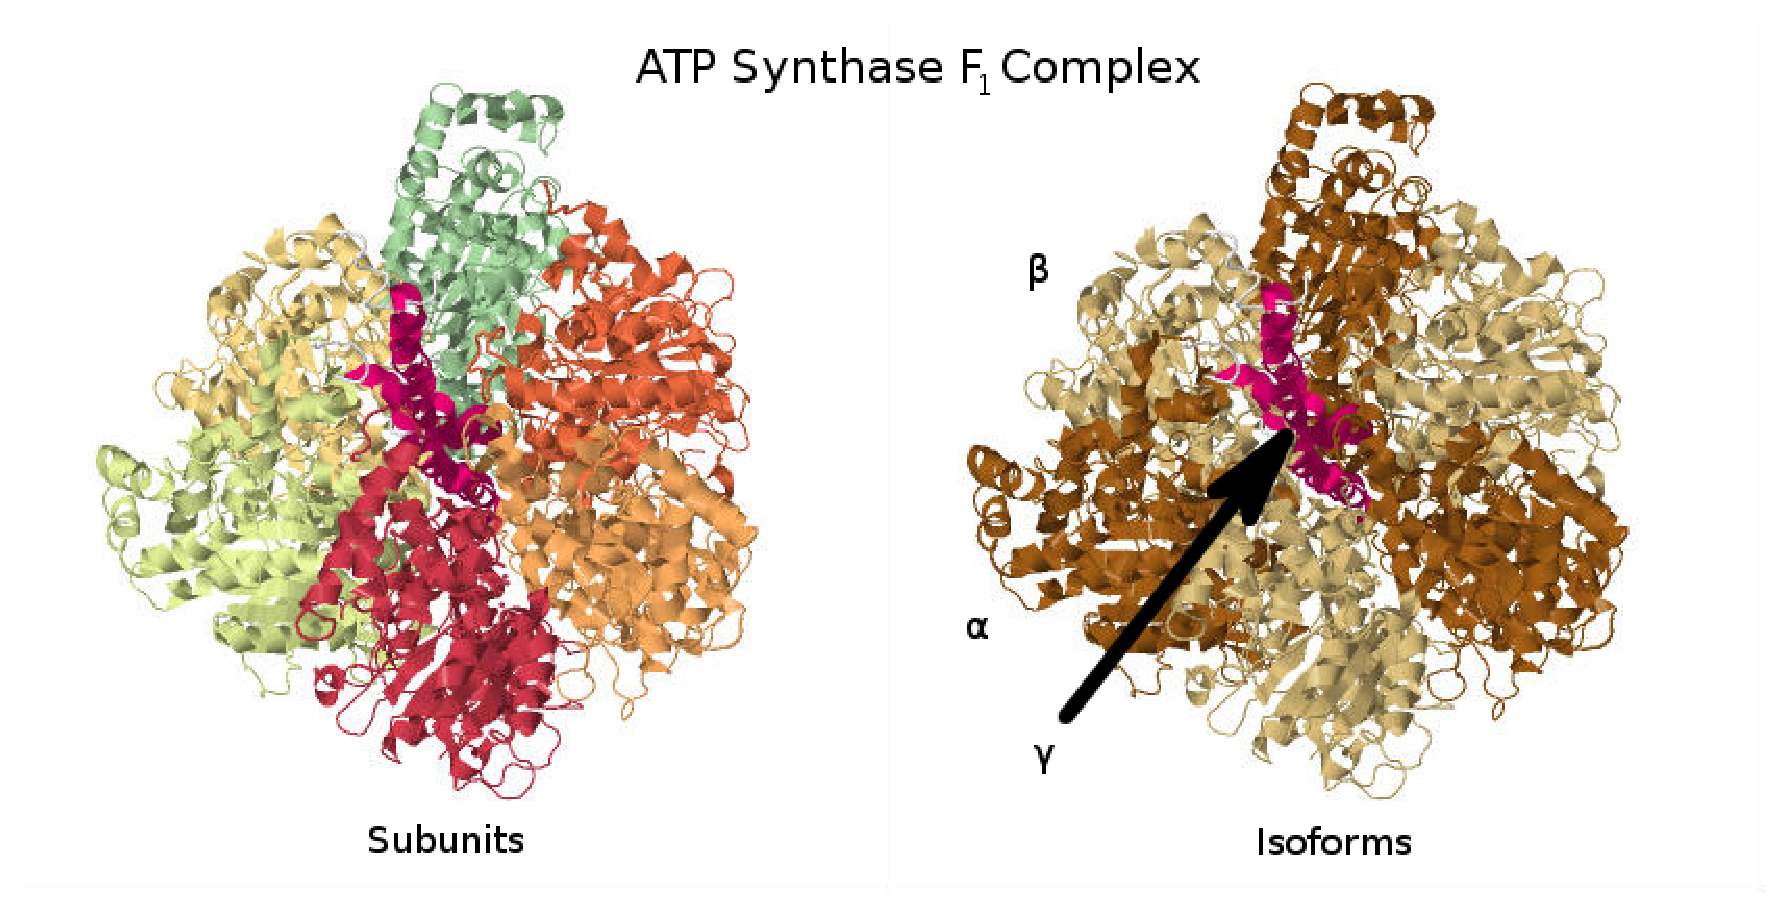
\includegraphics[clip=true,trim=0cm 0cm 0cm 0cm, width=12cm]{2F43}
\end{figure}

\emph{Assumption~\ref{ass:hierarchy}.}
The modeling of enzyme complex copy number can be tackled by using
nested sets of subcomplexes; each enzyme complex consists of multiple
subcomplexes, unlesss it is only a single protein or family of protein
isozymes.  These subcomplexes are required for the enzyme complex to
function (AND relationships), and can be thought of as the division of
the complex in to distinct units that each have some necessary
function for the complex, with the exception that we do not keep track
of the multiplicity of subcomplexes within a complex since this
information is, in the current state of affaris, not always known.
However, there may be alternative versions of each functional set
(given by OR relationships). Eventually, this nested embedding
terminates with a single protein or set of peptide isoforms
(e.g. isozymes).  In the case of ATP Synthase, one of its functional
sets is represented by the $F_1$ subcomplex. The $F_1$ subcomplex
itself can be viewed as having two immediate subcomplexes: the single
$\gamma$ (axel) subunit and three identical subcomplexes each made of
an $\alpha$ and $\beta$ subunit. Each $\alpha\beta$ pair works
together to bind ADP and catalyze the reaction (cite). The
$\alpha\beta$ subcomplex itself then has two subcomplexes composed of
just an $\alpha$ subunit on the one hand and the $\beta$ subunit on
the other.  It is obvious that one of these base-level functional
subcomplexes (in this example, either $\gamma$ or $\alpha\beta$) will
be in most limited supply, and that it will best represent the overall
enzyme complex copy number (discounting the issues of multiplicity for
$\alpha\beta$, discussed above).

%
% Consider adding this as a Theorem/Proof:
%

The hierarhical structure just described, when written out in Boolean,
will give a rule in CNF (conjunctive normal form). This is because all
relations are ANDs (conjunctions), except possibly at the inner-most
subcomplexes that have alternative isoforms, which are expressed as
ORs (disjunctions). Since GPR rules alone only specify the
requirements for enzyme complex formation, we will see that not all
forms of boolean rules are equally useful in evaluating the enzyme
complex copy number, but we have established assumptions
~\ref{ECAssume} and an alternative and logically equivalent rule
\hl{(cite logic book)} under which we can estimate enzyme complex copy
number.

\hl{Consider adding one more illustrative figure for these CNF<-> enzyme complexes (before sending to Mike).}

% !!!!!!!!!!!!!!!!!!!!!!!!!!!!!!!!!!!!!!!!!!!!!!!!!!!!!!!!!!!!!!!!!!!!
% Need to discuss each assumption in turn. Maybe emphasize the text at the 
% start of each paragraph with e.g. \emph{Assumptions 4-5}.
% !!!!!!!!!!!!!!!!!!!!!!!!!!!!!!!!!!!!!!!!!!!!!!!!!!!!!!!!!!!!!!!!!!!!

\label{ECAssume}
\begin{center}
\begin{tabular}{| p{14cm} |}
\hline
\textbf{Box ~\ref{ECAssume}. Assumptions in GPR-based Enzyme Complex Formation} \\
\hline
\begin{enumerate}
\item \begin{assume} \label{ass:expcorr}
Expression values are highly correlated the copy numbers of their
corresponding peptide isoforms.
\end{assume}
\item \begin{assume} \label{ass:isozyme} 
Protein isoforms contributing to isozymes are considered part of the
same enzyme complex.
\end{assume}
\item \begin{assume} \label{ass:hierarchy}
Any enzyme complex can be described as a hierarchical subset of
(possibly redundant) subcomplexes; redundant subcomplexes, as
elaborated in (\ref{ass:nostoich}), are not currently modeled.
\end{assume}
\item \begin{assume} \label{ass:nostoich} 
Assumes one copy of peptide per complex; exact isoform stoichiometry
is not considered.
\end{assume}
\item \begin{assume} \label{ass:sharing} 
With the exception of complexes having identical rules (i.e. the same
complex listed for different reactions), assume each copy of a peptide
is available for all complexes in the model.
\end{assume}
\item \begin{assume} \label{ass:holo} 
If a particular subcomplex can be catalyzed by A and it can also be
catalyzed by A and B (e.g. B acts as a regulatory unit, as in
holoenzymes), this just simplifies to A once expression values are
substituted in. Similarly, allosteric regulation is not
modeled. Relately, there are no NOT operations in GPR rules (just ANDs
and ORs). However, cofactors may be considered separately in the
corresponding reaction stoichiometry.
\end{assume}
\end{enumerate} \\
\hline
\end{tabular}
\end{center}

There is no gaurantee a GPR rule has been written down with this
hierarchical structure in mind, though it is likely the case much of
the time as it is a natural way to model complexes.  However, any GPR
rule can be interpreted in the context of this hierarchical view due
to the existence of a logically equivlaent CNF rule for any non-CNF
rule, and it is obvious that logical equivalence is all that is
required to check for enzyme complex formation when exact isoform
stoichiometry is unknown.  As an example, we consider another common
formulation for GPRs, and a way to think about enzyme
structure---disjunctive normal form (DNF).  A DNF rule is a
disjunctive list of conjunctions of peptide isoforms, where each
conjunction is some variation of the enzyme complex due to
substituting in different isoforms for some of the required
subunits. A rule with a more complicated structure and compatible
isoforms across subcomplexes may be written more succinctinly in CNF,
whereas a rule with only very few alternatives derived from isoform
variants may be reprsented clearly with DNF.  In rare cases, it is
possible that a GPR rule is written in neither DNF or CNF, perhaps
because neither of these two alternatives above are stricly the case,
and some other rule is more succinct.

\emph{Assumptions~\ref{ass:nostoich}~and~\ref{ass:sharing}.}
Note that it is possible for an enzyme complex to catalyze different
reactions. In fact, some transporter complexes can transfer many
different metabolites \hl{across a lipid bilayer--up to}. Another
example is the ligation or hydrolysis of nucleotide, fatty acid, or
peptide chains, where chains of different length may all be substrates
or products of the same enzyme complex. While we do not explicitly
consider these in Algorithm~\ref{alg:ReductionToCNF}, these
redundancies are taken into account subsequently in
Algorithm~\ref{alg:eMoMA}.  What is currently not considered in our
process is that some peptide isoforms may find use in completely
different complexes; in this case, we assume an unrealistic case of
superposition where the isoform can simultaneously function in more
than one complex. The primary reason we have not tackled this problem
is because exact subunit stoichiometry of most enzyme complexes is not
accurately known, but an increasing abundance of data on BRENDA gives
some hope to this problem \hl{(cite BRENDA)}.

\emph{Assumption~\ref{ass:holo}.}
We do not make any special assumptions requring symmetry of an isoform
within a complex. For instance, the example in
assumption~\ref{ass:holo} shows how you might have one
subcomponent composed of a single isoform, and another subcomponent
composed of that gene in addition to another isoform. In this case, it
is simply reduced to being the first gene only that is required, since
clearly the second is strictly optional. That isn't to say that the
second gene may not have some effect, such as (potentially) aiding in
structural ability or altering the catalytic rate, but it should have
no bearing on the formation of a functional catalytic
complex. Holoenzymes---enzymes with metabolic cofactors or protein
subunits that have a regulatory function for the complex---would
likely be the only situation where this type of rule might need to be
considered in more detail. But in the absence of detailed kinetic
information, this consideration not be useful, much like allosteric
regulation.

\subsection{Orignal eMoMA Formulation}

The prior work does not use an acronym for labeling their method \cite{Lee2012}.
However, their work was a direct inspiration for the current approach, 
so we also consider this a form of eMoMA. Please also see this paper for examples
of mapping gene expression data to expression and variation of enzyme complex
copy number.

\subsection{Motivational Gene-Rule Examples for\\ Conjunctive Normal Form}
The previous direct evaluation of gene rule expression values can lead to some problems.
Below, lower case letters denote expression level (i.e. copy number of mRNA) of their
corresponding upper case letter, which denotes the gene name. The $r_i$ are different reaction
rules and the $e_i$ are the corresponding estimated complex expression levels.

We need some way to guarantee that we don’t count anything twice or more across disjunctions: \\
\begin{tabular}{cccccccc}
& $r_1$ & := & [A and B] or [A and C] & $\rightarrow$ & $e_1$  &=& min($a,b$) + min($a,c$) \\ 
& $r_2$ & := & [A and (B or C)]       & $\rightarrow$ & $e_2$  &=&  min($a, b + c$) 
\end{tabular} \\
Supposing A is the minimum, then if we just evaluate $r_1$ directly (a rule in 
disjunctive normal form, or DNF), A will be counted twice. 

Another possibility is divvying up expression as seen in DNF. For instance, in $r_1$ above,
we could evaluate it as $e_1$ = min($\frac{a}{2},b$) + min($\frac{a}{2},c$) to account for
the repeated use of $a$. However, other potential issues aside, we can see that this can
cause problems rather quickly. For instance, suppose $b = a$ and $c = 0$; then min($a$,$b+c$) 
$=b=a$ appears to be correct, not min($\frac{a}{2},b$) + min($\frac{a}{2},c$) = $\frac{a}{2} + 0$. 

Attempting to symbolically convert the human ATP Synthase rule in
Human Recon 2 to CNF is computationally intractable due to an
exponential increase in memory \cite{Thiele2013}. Therefore, we use a
reduction rule that makes use of expression data, outlined below. The
algorithm can be represented as follows: \\

\pagebreak
\begin{Algorithm}
\label{alg:ReductionToCNF}
\begin{algorithmic}
\REQUIRE $g_i$ are genes. 
\REQUIRE $x_i$ are expressions in Boolean logic.
\WHILE{$rule \neq AND(o_1,...,o_n)$ where $o_i$ has the form: $OR(g_1,...,g_m)$}
  \STATE $\mathbf{1}$: check for sequence of ANDs of literals (genes)\\ 
    \hspace{4.8 mm} $\rightarrow$ reduce to gene with minimum expression 
  \STATE $\mathbf{2}$: Distribute ORs over ANDs, e.g.: $(x_1 \land x_2) \lor (x_3 \land x_4)$ \\ 
    \hspace{4.8 mm} $\rightarrow (x_1 \lor x_3) \land (x_1 \lor x_4) \land (x_2 \lor x_3) \land (x_2 \lor x_4)$
  \STATE $\mathbf{3}$: Change adjacent gene arguments to sets, e.g: \\
    \hspace{4.8 mm} $g_1 \land g_2 \rightarrow AND(g_1,g_2)$;  \\
    \hspace{4.8 mm} $g_1 \land AND(g_2,g_3) \rightarrow AND(g_1,g_2,g_3)$ 
\ENDWHILE
\ENSURE $o_{min}$ where $o_{min}$ has the form: $OR(g_1,...,g_m)$
\end{algorithmic} 
\end{Algorithm}

The third step greatly simplifies numeric manipulations and checking
for the terminating condition. Please see below for the code for the
core part of the algorithm. Now we show that the reduction step does
not change the desired result of the algorithm.

\begin{Theorem}
\label{thm:ReductionToCNF}
Algorithm~\ref{alg:ReductionToCNF} returns the disjunction with
minimum expression value among all disjunctions of a rule in CNF.
\end{Theorem}

\begin{proof}
The third step in the while-loop does not affect the
underlying logic, so we only need to consider the effect of step one
on step two.  Let us first consider when expressions $x_1, ..., x_4$
are all literals in step two to cover the most complex case, and that
$x_i^{(e)}$ denotes the expression measurement for gene $x_i$. Assume
WLOG that $x_1 \lor x_3$ attains the minimum expression among the
disjunctions. Then we have:

\begin{align*}
&x_{1}^{(e)} + x_{3}^{(e)} \leq x_{1}^{(e)} + x_{4}^{(e)} \Rightarrow x_{3}^{(e)} \leq x_{4}^{(e)} \\
&x_{1}^{(e)} + x_{3}^{(e)} \leq x_{2}^{(e)} + x_{3}^{(e)} \Rightarrow x_{1}^{(e)} \leq x_{2}^{(e)} 
\end{align*}

Applying this result in conjunction to step one in the while-loop to
the original expression, $(x_1 \land x_2) \lor (x_3 \land x_4)$, we
immediately arrive at $(x_1) \lor (x_3)$, which gives our originally
assumed minimum. To show that this result doesn't depend on the $x_i$
being literals, merely consider repeating this process recursively for
each $x_i$ that is not a literal to arrive at two different
evaluations for $x_i^{(e)}$. Since the process cannot continue
indefinitely, eventually there is a base case involving only literals,
and the above result shows that both evaluations will be
identical. Propagating back will yield the desired result. Because
Algorithm~\ref{alg:ReductionToCNF} without step one simply yields CNF,
it follows that adding step one will yield the disjunction with 
minimum expression value of the rule in CNF.
\end{proof}

The method presented here for enzyme complex copy number estimation can be used as a stand-alone method,
as long as GPR rules from a metabolic reconstruction are present. For instance, it 
may not always be desirable to directly compute a flux. As an example, the relative copy number of
enzyme complexes present in secretions from various biological tissues, such as milk or pancreatic
secretions. Perhaps more importantly, this approach to estimating relative complex levels can be employed
with regulatory models such as PROM or other regulatory network models that can estimate individual gene
expression levels at time $t+1$ given the state of the model at a time $t$ (cites PROM, some other bayesian
regulatory/signalling model).

\subsection{Formulation with Automatic Normalization and Fast Direction Assignment}
Unlike the original formulation of eMoMA, we employ a normalization variable $n$ in the problem
to find the most agreeable scaling of expression data. Additional technical constraints not shown
from Linear Fractional Programming (LFP) require $n$ to be non-zero \cite{Boyd2004}. The
LFP shown below can be converted to a linear program by the Charnes-Cooper transformation.

Additionally, the original formulation
used repeated iterations of FVA (Flux Variability Analysis). This is a very costly procedure. 
To address this, we convert the model to an irreversible model, where each reversible flux $v$
in the original model is split into a forward and backward reaction that take strictly positive
values: $v_f$ and $v_b$. Given an indexed family $R$ of reactions with the identical gene rules in each
set and estimated expression values $e_i$, we can describe the new problem as:

\vspace{5 mm} 
\hl{(Need to describe iterative process in Algorithm.)}
\begin{Algorithm}[eMoMA]
\label{alg:eMoMA}
\begin{align*}
&\textnormal{minimize}\ \sum^N_{i=1}\frac{d_i}{n \sigma_i}  \\
&s.t. \\
&\forall i: -d_i \leq \sum_{j \in R_i}(v_{j,f} + v_{j,b}) - n e_i \leq d_i \\
&d_i \geq 0 \\
&n > 0
\end{align*}
\end{Algorithm}
Note that as in the original eMoMA paper, $\sigma_i$ is an optional weighting of variation
in biological or technical replicates. 

In the original formulation, FVA uses an objective with a $-1$ or $+1$ for each reversible reaction 
with all other reactions having a 0. If having a non-zero flux in the negative or positive direction
does not increase the residuals' magnitude (which is the objective of the eMoMA problem), then 
the reaction is made irreversible for subsequent iterations. Eventually this process terminates
when the number of reversible reactions remains constant. 

During each iteration we allow flux through both $v_f$ and $v_b$; if one of these is is greater 
than the other, then the lesser flux is constrained to be zero in subsequent iterations. What
can be done in practice is to pick a parameter $\alpha \in [0.5,1)$ so that if
$\frac{v_f}{v_f+v_b} > \alpha$ then $v_b$ is constrained to be 0 subsequently. This parameter could
also be changed as iterations progress, but so far there appears to be no advantage to using
anything other than $0.5$ (larger values terminate more quickly, but with slightly fewer reaction
directions determined).

If $v_f = v_b$ after an iteration, we constrain both reactions to be zero, since this
is a futile cycle. Otherwise, the flux through these reactions may be inadvertently affecting
the obective. If we don't do this, we actually see about 100 fewer reactions active in an eMoMA run.
The disadvantage is that the time for completing eMoMA goes up from about 70s to 200s on a recent
AMD Athlon Magny-Cours system running the Gurobi 5.1 solver. This is still a major improvement 
in efficiency over the FVA method, which could take several hours per Human Recon 2 eMoMA run.

Futher work on improving convergence speed should be kept in mind, or at least, making use of prior
eMoMA flux estimations (see the section below about mutational models and epistasis).

\subsection{Applications and Insights from GPR formalisms and eMoMA}
When should an investigator simply look at gene expression levels rather than
worrying about the additional complexities of GPRs and flux estimation as in eMoMA?
Perhaps the most obvious example is attempting to estimate actual enzyme-catalyzed 
fluxes rather than expression levels, since individual gene expression levels
may not be straight-forward to draw conclusions from due to non-linearities
from the GPRs, as well as network-related effects. Additionally, methods like these
allow us to impute fluxes for reactions that are not catalyzed by enzymes,
such as transport reactions or highly spontaneous chemical reactions. To illustrate
this point, Table XXXX shows the correlation matrix for the above quantities and 
the distributions of each quantity for a single eMoMA run (XXXX).

\section{Discussion}
We have formalized and improved an existing method for estimating flux
from expression data, as well as listing assumptions in the model that
may be useful to address in later attempts ~\ref{ECAssume}. Another
caveat is that GPR rules or stoichiometry may be inaccurate or
incomplete in any given model. In fact, for the forseeable future,
this is a given. By using the GPR and not just the stoichiometry to
estimate flux, it is possible that future work could make use of this
framework to debug not just stoichiometry as some methods currently do
\hl{(cite e.g. grow match, etc.)}, but also GPR rules.

\section{Future Analysis}
\subsection{An Analysis of Cancer Tissue Metabolism}
\subsection{Cancer's Influence on Nighboring Tissue}
\subsection{Epistasis Extended to Beneficial Mutations and Non-Microbial Models}

The occurence of beneficial mutations and how they affect adaptation is currently an area of active
interest in evolutionary biology \cite{Chou2011} \cite{Weinreich2006}. The questions are often difficult
or impossible to assess experimentally due to limited resources.  In genome-scale models, to our knowledge,
only microbial epistasis has so far been studied for all enzymes (often referred to as genome-scale 
in this context). This is due to several factors.

One issue is that these computations can still take a significant amount of time, and the increase in model
size of Human Recon 2 over Yeast can cause even a relatively simple FBA run to go up by an order of magnitude.
This problem is compounded by the increase in the number of genes in the human model, since computing epistasis
consumes space and time as $O(n^2)$ where $n$ is the number of genes in the model. More important than this issue,
which might be overcome with enough computational resources, is the issue of an objective function. It has been shown
numerous times that FBA with a biomass objective can be a reasonable approximation to what a microbe is trying to 
achieve metabolically ~\cite{Schuetz2012}~\cite{Fong2004}~\cite{Varma1994} . While Recon 2 is equipped with a ``generalized biomass reaction'', it is not clear
what the meaning of this is, and it certainly seems unlikely to estimate the metabolism even of fast-growing cancer
cells \hl{(cite Locasale?)}. We propose eMoMA as a method to get around this issue for non-microbial models.

Another advantage to eMoMA is that it allows one to directly probe mutations that are represented as gene expresion
perturbations. A decreased level of gene expression may also be metabolically equivalent to the effect of a missense
mutation, for example. This allows a different sampling strategy than before; for instance, we could observe how uniform 
expression restriction compares to uniform flux restriction~\cite{Xu2012}. Assuming an accurate model of enzyme-complex
expression measurement, the former should be the more realistic model.

One issue discussed elsewhere is that combining traditional flux restriction mutations, which are known as 
\emph{hard constraints}, may result in an unsolvable system, which is almost certainly an undesired effect
of this mutation modeling formalism. Instead, it would be better if mutations could be modeled as 
\emph{soft constraints}. Concretely, whereas hard constraints are enacted in the actual constraints of the 
optimization problem, soft constraints merely change the objective. This means that multiple soft constaints
combined together under some mutational model would be compatible in the sense that they wouldn't unexpectedly
result in an unsolvable system. eMoMA provides two possible avenues for soft constraints: expression level 
and expression variation. \emph{However, it is not clear yet what expression variation really means, so further
investigation is necessary.}

\section{Code}
\subsection{minDisjunction}

The following code is written in ATS, a type-safe language including syntax similar to SML while
having direct access to C types \cite{ATStypes03}.
GREXP describes a datatype that is used for storing the parse trees of Boolean rules (without negation).
A GREXP can then be manipulated by the function toCNF to be converted to a conjunctive normal form.
We make use of the reduction rule mentioned previously by calling the minConj function. The 
conjunctivize function is a helper function to deal with different structures for a GRconj
and GRdisj (one is set based, one is parse-tree based; note this described in the data(view)type defintion).

\begin{verbatim}
dataviewtype GREXP = 
  | GRgenes of genes
  | GRconj of genes
  | GRconj of (GREXP,GREXP)
  | GRdisj of genes
  | GRdisj of (GREXP,GREXP)

extern
fun toCNF (bexp: GREXP, emap: &gDMap): GREXP

implement
toCNF (bexp, emap): GREXP = let     
  val LR:GREXP = (case+ bexp of 
    | ~GRconj(ex1,ex2) => GRconj (toCNF(ex1,emap),toCNF(ex2,emap))
    | ~GRdisj(ex1,ex2) => GRdisj (toCNF(ex1,emap),toCNF(ex2,emap))   
    | GR => GR):GREXP
  in (case+ LR of  
    | ~GRconj(ex1,ex2) => minConj(GRconj(ex1,ex2),emap) 
    | ~GRdisj(ex1,ex2) => (case+ (ex1,ex2) of
      // Handle disjunctive leaf cases:         
      | (~GRdisj(lx), ~GRgenes(g)) => GRdisj (lx + g) 
      | (~GRgenes(g), ~GRdisj(rx)) => GRdisj (rx + g)
      | (~GRdisj(lx), ~GRdisj(rx)) => GRdisj (lx + rx)
      | (~GRgenes(g1), ~GRgenes(g2)) => GRdisj (g1 + g2)

      // Distribute OR over ANDs:
      | (~GRconj(x1,x2), ~GRconj(g)) => conj1(x1,x2,g,emap) 
      | (~GRconj(g), ~GRconj(x1,x2)) => conj1(x1,x2,g,emap) 
      | (~GRconj(g1), ~GRconj(g2)) => conj2(g1,g2,emap)
      | (~GRconj(lx1,lx2), ~GRconj(rx1,rx2)) => let
        val lx1c = GREXP_copy(lx1)
        val lx2c = GREXP_copy(lx2) 
        val rx1c = GREXP_copy(rx1)
        val rx2c = GREXP_copy(rx2) 
        in GRconj(GRconj(GRconj(toCNF(GRdisj(lx1,rx1),emap), 
          toCNF(GRdisj (lx2, rx1c ),emap)),
          toCNF(GRdisj (lx1c, rx2),emap)), 
          toCNF(GRdisj (lx2c, rx2c),emap)) 
        end

      // Handle e.g.: (.. OR ..) OR (.. AND ...) 
      | (~GRconj(lx1,lx2), RX) => let
        val RXc = GREXP_copy(RX)
        in GRconj(toCNF(GRdisj(lx1,RX),emap),
          toCNF(GRdisj(lx2,RXc),emap)) 
        end
      | (LX ,~GRconj(rx1,rx2)) => let
        val LXc = GREXP_copy(LX)
        in GRconj(toCNF(GRdisj(LX,rx1),emap),
          toCNF(GRdisj(LXc,rx2),emap)) 
        end
      | (~GRconj(gc), RX) => let
        val retGR = toCNF(conjunctivize(RX, gc,emap),emap)
        val _ = genes_free(gc)
        in retGR end
      | (LX, ~GRconj(gc)) => let
        val retGR = toCNF (conjunctivize(LX, gc,emap),emap)
        val _ = genes_free(gc)
        in retGR end
      // All other disjunctive cases
      | (_,_) => GRdisj(toCNF(ex1,emap),toCNF(ex2,emap))
      ):GREXP
    | EX => EX
    ):GREXP
  end
\end{verbatim}


\chapter{Cancer Phenotypes and eMoMA}

\appendix
\chapter{Chapter 1 of appendix}
Appendix chapter 1 text goes here

\bibliography{dissertation}

\end{document}
